
\section{Introduction}
% OPENING - DEMOCRACY 
Democracies face two big problems. First, they are vulnerable to fleeting passions and demagogues. To combat this, they leave many decisions to experts who, ideally, use wisdom and judgment loosely guided by the public. Second, everyone cannot vote on every decision. Thus, they delegate power to representatives (who then delegate it to deputies), create temporary mini-publics,
and solicit input from those most affected or moved by a public decision.\footnote{
As imagined by \citet{Dahl1989}, mini-publics are representative, selected at random, and deliberative. Besides juries, however, deliberative and randomly-selected bodies are rare. Instead, citizens more often engage in government decisions when given opportunities to opt-in, such as hearings, petitions, and public comment periods. These mechanisms of engagement generate a different, more contentious flavor of public input.
}
Most policy is then made by bureaucrats, supposedly guided indirectly through elected representatives and directly by limited public input (mostly on highly contentious policies).
By one estimate upward of 90\% of legally binding U.S. federal policy is now written by agencies \citep{West2013}.

% Both of these problems converge in the bureaucracy, run by experts who are deputized by elected officials (or by their deputy's deputy's deputy) and with procedures that create opportunities for public input. It is far from clear how bureaucratic decisions are to balance expertise, accountability to elected officials, and responsiveness to public input in decisionmaking. 

Expertise, delegation, and limited public input thus converge in bureaucratic policymaking, where bureaucrats are required to use reasoned judgment, be accountable to elected officials, and be responsive to public input. There is no normative consensus on how to rank or merge these aims.
Administrative procedures for gathering input and their justifications cite all three.



% MODELS HAVE NO PLACE 
Leading models of bureaucratic policymaking focus on how agencies either learn about policy problems, negotiate or avoid accountability to various principals, or balance interest-group demands.\footnote{
On learning, see \citet{Libgober2018} for an information-based model where commenting reveals information to the agency. 

On accountability to elected officials, see  \citet{Furlong1997}, \citet{Nou2016}, \citet{Potter2016}, \citet{Woods2018}, and \citet{Yackee2009RegGov}. For example, \citet{Potter2014dis} presents a signaling model where agencies propose and principals veto rules depending, in part, on their beliefs about interest group preferences. 

On interest group balancing see \citet{Yackee2006JOP},  \citet{Yackee2006JPART}, and \citet{Kerwin2011}.
} 
The contentious politics that inspire ordinary people to engage have no place in these models and have largely been ignored by political scientists, leaving a weak empirical base for normative and prescriptive work.


% \subsection{Why study rulemaking?}
% \section{The Importance of Studying Rulemaking}
% Mobilization may increasingly target rulemaking because it is how most policy in the U.S. is now made. 
With the rise of the administrative state in the United States, federal agencies have become a major site of policymaking and political contestation. In the years or decades between legislative enactments, federal agencies make legally-binding rules interpreting and reinterpreting old statutes to address emerging issues and priorities. %Ninety percent of new policy that carries the force of law is now made in the bureaucracy rather than in Congress \citep{West2013WhoControl}.\footnote{I use policy, law, and regulation as nested concepts. My methods generally apply to all policy texts whether they carry the force of law or not. Many public and private organizations, including agencies, have policy statements that are not legally binding. My empirical subject is rules that do carry the force of law based on some authorizing legislation. I use rule (a more technical term) and regulation (a more colloquial term) interchangeably.}
Examples are striking: %the effect of the Dodd-Frank Wall Street Reform and Consumer Protection Act was largely unknown until the specific regulations were written, and it continues to change as these rules are revised. 
Congress authorizes billions in farm subsidies and leases for public lands, but who gets them depends on agency policy. In the decades since the last major environmental legislation, agencies have written thousands of pages of new environmental regulations and thousands more changing tack under each new administration. Agency rules are revised more often than legislation \citep{Wagner2017DynamicRulemaking}.
 And these revisions can be significant. In 2006, citing the authority of statutes last amended in the 1950s, the Justice Department's Bureau of Prisons proposed a rule restricting eligibility for parole. In 2016, the Bureau withdrew this rule and announced it would be requiring fewer contracts with private prison companies, precipitating a 50\% loss of industry stock value. Six months later, a new attorney general announced these policies would again be reversed, leading to a 130\% increase in industry stock value. %Like many rulemaking debates, industry and advocacy groups spent millions of dollars lobbying on this issue. Few rulemakings, however, receive this level of public and presidential attention. In the majority of rulemakings, few participate, and we do not really know the extent to which participants get what they lobby for.% (but see Yackee and Yackee 2006)
Rulemaking clearly matters.

Less clear, however, is what the new centrality of agencies and rulemaking means for the practice of American democracy. In addition to the complex relationships agencies have with the president and Congress, agencies have complex and poorly understood relationships with the public and advocacy groups. Relationships with constituents may even provide agencies a degree of ``autonomy'' from their official principals \citep{Carpenter2001}. While some suggest that requirements for agencies to solicit and respond to public comments on proposed rules allows ``civil society'' to provide public oversight, others note that participants in rulemaking often represent elite parts of society \citep{Seifter2016ComplementaryPower} and business interests \citep{Yackee2006a}. Yet agency decisions are also the target of advocacy campaigns.\footnote{For example, along with 50 thousand protesters in Washington D.C., the State Department Received 1.2 million comments on the Environmental Impact Statement for the Keystone Pipeline. Similarly, along with the thousands of protesters supporting the Standing Rock Sioux protest to the Dakota Access Pipeline, the Army Corps of Engineers received hundred of thousands of comments. Along with 22 million comments on the Federal Communications Commission's Open Internet rules, activists are organizing online protest actions. On each of these issues, advocacy activity has been followed by legislative or executive action.} 

Agencies advertise public comment periods as an opportunity for a voice in government decisions.\footnote{
% FOCUS
I focus on public comments in rulemaking, but my theory and methods also apply to other kinds of political engagement such as through social media or protests as well as to other political decisions, including state-level rulemaking. Social media engagement may be especially important if agencies implement the recommendations of \citet{ACUS2018} that ``Agencies should consider using social media before or in connection with direct final rulemaking to quickly identify whether there are significant or meaningful objections'' (p. 34). 
} 
%The notice-and-comment process purports to be an avenue of citizen voice. 
Big red letters across the top of the Regulations.gov homepage solicit visitors to ``Make a difference. Submit your comments and let your voice be heard.'' A blue "Comment Now!" button accompanies a short description of each draft policy and pending agency action. 
Commenting on proposed agency rules is described as ``an important part of democracy'' (WSJ 2017), the ``purest example of participatory democracy in actual American governance'' \citep{Herz2016}. \citet{Rossi1997} finds that ``courts, Congress, and scholars have elevated participation [in rulemaking] to a sacrosanct status...greater participation is generally viewed as contributing to the democracy.'' % Is it?
 While most rules receive little attention, the ease of online commenting and mobilizing has created exponential increases in the number of rules where which hundreds of thousands of citizens participate (see figure \ref{fig:comments}). Occasionally, large numbers of citizens are paying attention.

\begin{figure}[!hb]
\caption{Number of Public Comments Total (Left) and Under 1 Million (Right). The most commented on rules have been published by the Federal Communications Commission (FCC, omitted from this plot), the Environmental Protection Agency (EPA), the Department of Interior (DOI), the Bureau of Ocean Energy Management (BOEM), the Consumer Financial Protection Bureau (CFPB), and Fish and Wildlife Service (FWS).}
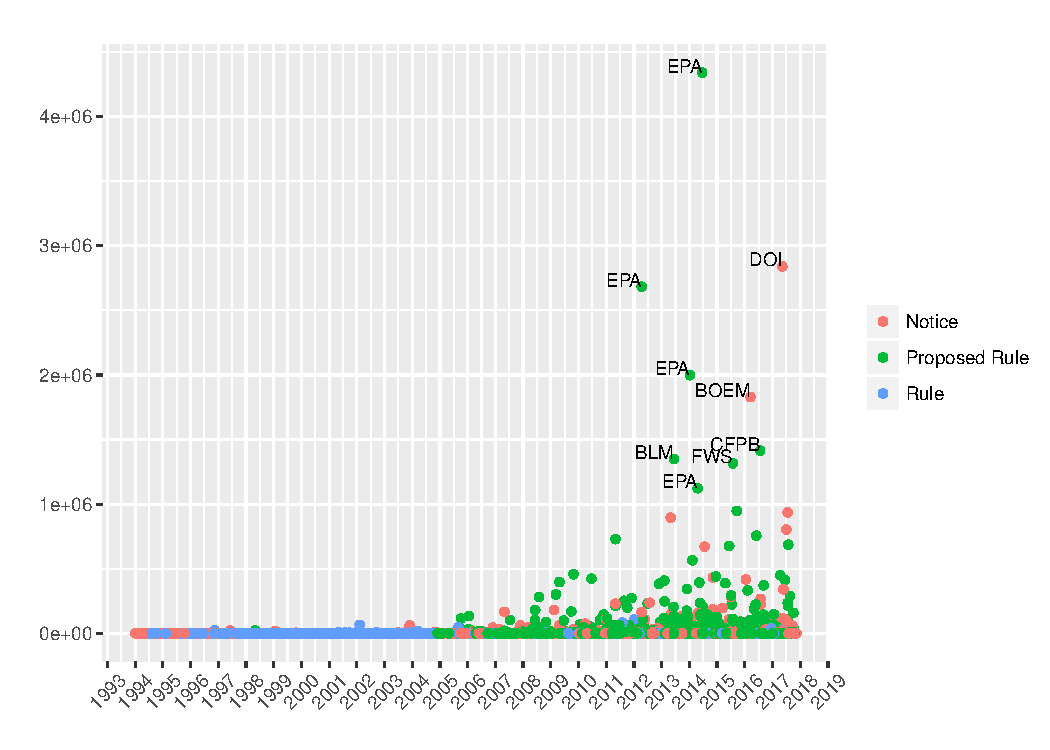
\includegraphics[width= 3.5in]{number_of_comments.pdf}
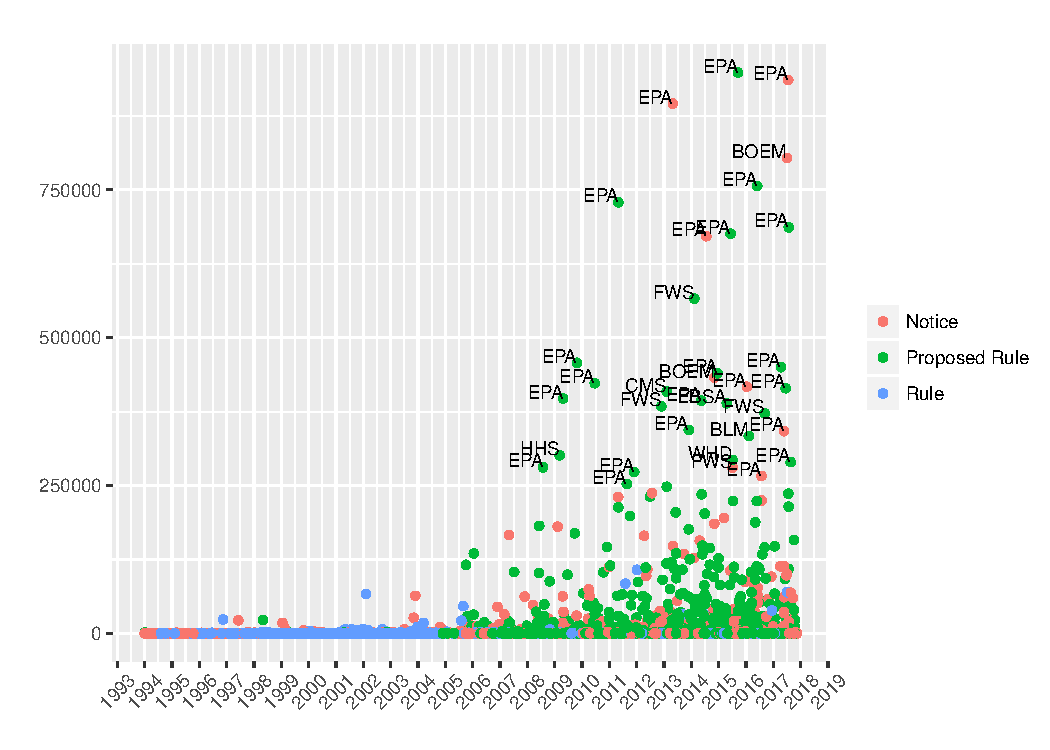
\includegraphics[width = 3.5in]{comments_under_1m.pdf}
\label{fig:comments}
\end{figure}

%It is even less clear whether actions by average citizens make a difference in agency policymaking. Many may believe that they do, but the mechanisms are not obvious. Indeed letter writing and other forms of mass mobilization do not have a clear place in political scientists' theories of bureaucratic politics. This lack of scholarship may be the result of both a general suspicion, rooted in certain theories of strategic behavior, that mass politics affects unelected career officials as well as a normative assumption that policy ``implementation'' is no place for contentious politics. Neither the bureaucrat who asserts that rules are the result of scientific analysis nor the political scientist who asserts that rules are the result of bureaucrats strategically selecting their most preferred policy within institutional constraints offer an explanation for why an agency would receive millions of public comments or why they would matter.




% LEGAL SCHOLARS' DEBATES 
Legal scholars have long debated what to make of mass commenting in rulemaking. Many focus on reforms for agencies to collect more useful information \citep{Farina2011, Farina2014, Rauch2016}. In 2018, ``Public engagement'' was main project of the Administrative Conference of the United States (ACUS) committee on Rulemaking: \href{https://www.acus.gov/research-projects/public-engagement-rulemaking}{The project} ''explores agency strategies to enhance public engagement prior to and during informal rulemaking. It seeks to ensure that agencies invest resources in a way that maximizes the probability that rulewriters obtain high quality public information.''  Among other things, this committee is debating how to encourage ``quality public information,'' how ``to get new people/groups into the real or virtual room'' \citep{Farina2018}, and whether broad engagement is even desirable on all rules \citep{White2018}. \citet{Mendelson2011} finds that agencies often discard non-technical comments but argues that they should be given more weight. Others worry that mass commenting distracts agencies from good policy and the broader public interest \citep{Coglianese2006}. \citet[p. 112]{Farina2012} argues that ``[Mass] comments typically are neither factually informative nor reliable indicators of citizens’ informed value preferences.'' \citet{Rossi1997} argues it should be largely eliminated. \citet[p. 208]{Herz2016} concludes ``The goal of e-rulemaking is to more fully capture such credible, specific, and relevant information, not to solicit the views of random, self-nominating members of the public.'' Even scholars suggesting reforms aimed at ``regulatory democracy'' aim to increase the ``sophistication'' of ordinary peoples' comments \citep{Cuellar2015}. I argue that scholars focusing on deliberation have overlooked the role importance of political information and representation (but see \citet{Reich1966} and \citet{Seifter2016UCLA} on representation).
Notably, the ACUS draft recommendations on ``Mass and Fake Comments in Agency Rulemaking'' suggests that ``effective comments'' give ``reasons rather than just reactions'' \citep[p. 33]{ACUS2018}. If true, public reactions to proposed rules such as mass comments would have no effect in rulemaking. 

% MAY NOT MATTER 
Like most forms of political participation, 
mass public comments on draft agency rules provide no new technical information. 
They lack the authority of elected officials' opinions. 
And the number on each side has no legal import for an agency's response.
Policymakers may very well pay no attention to them. 

% SOPHISTICATED LOBBYING
Instead, scholars focus on the sophisticated lobbying efforts of powerful interest groups, whose role in shaping policy has been theoretically developed and empirically tested.
Foundational scholarship on rulemaking by \citet{Furlong2004}, \citet{Furlong1997, Furlong1998}, and \citet{Kerwin2011} focuses on interest group lobbying. Both theory and empirical scholarship suggest skepticism that the input of ordinary people matters. 
% REREAD BERRY
% \citet{Berry1999TheGroups} argues that mass engagement occurs too late in the policy process to be effective compared to insiders who are able to shape agendas and alternatives. 
Empirical scholarship finds that economic elites and business groups dominate American politics in general \citep{Gilens2014} and rulemaking in particular \citep{Crow2015, Wagner2011, West2009, Yackee2006JOP, Yackee2006JPART, Yackee2012, Golden1998, Haeder2015}. Perhaps this is unsurprising. 
From a strategic perspective, agency officials are not directly accountable to voters. And even if organized groups do supplement congressional and judicial checks on executive power, the groups that participate in rulemaking represent only certain (if any) citizens and may not represent them well \citep{Seifter2016UCLA}. Early optimism among legal scholars that the internet would ``change everything'' \citep{Johnson1998} and that ``cyberdemocracy''  would enable more deliberative rulemaking has faded.  Here, the prediction that the internet would merely facilitate engagement among the like-minded \citep{Sunstein2001} has largely been correct. While commenting and encouraging others to comment has become easier, \citet{Coglianese2006} finds that little else has changed. 
From a science-based policy perspective, average citizens signing form letters provide no new information to policymakers. 
Mass comment campaigns are thus often called ``spam'' \citep{Balla2018} and dismissed as epiphenomenal to bargaining with principals or interest groups. 
Yet \citet{Yackee2015JPART} finds that, even though ordinary participants see business influence as more important, they still strongly believe that their comments matter.

% MAIN QUESTION 
% Yet agencies occasionally receive thousands or even millions of comments from ordinary people. %Why? 
How, if at all, should scholars incorporate mass engagement into models of bureaucratic policymaking? 
I argue that mass engagement produces political information about the coalition that mobilized it and thus, depending on how agencies process political information, ``going public'' may occasionally be an effective strategy for organizations to influence policy, both directly and indirectly.\footnote{
% DEFINITION
Political scientists often define civic engagement as writing to government officials, signing petitions, attending hearings, attending protests, or donate to a political campaign. While donating is more common in electoral politics, activists frequently attempt to influence agency policymaking through letter-writing, petitions, hearings, and protests. I suspect that mass commenting is driven by the same privileged populations known to engage in other civic activities. % Does it work? If so, by what mechanisms?

Following the conventional terms ``mass comment campaign'' and ``public engagement,'' I call the general phenomenon ``mass engagement'' resulting from ``mass mobilization'' in order to distinguish the magnitude of civic engagement.
By mass engagement, I mean that thousands of people beyond professional policy influencers engage. Contrary to the common assumption that this emerges organically, it is almost always mobilized by an organization that also engages in sophisticated lobbying. %\footnote{
As \citet{SantAmbrogio2018} conclude ``The `mass comments' occasionally submitted in great volume in highly salient
rulemakings are one of the more vexing challenges facing agencies in recent years. These comments are typically the result of orchestrated campaigns by advocacy groups to persuade members or other like-minded individuals to express support or opposition for an agency's proposed rule.''
}
% Representation 
Those lobbying in rulemaking often make suspect claims to represent broad segments of the public \citep{Seifter2016UCLA}. Mobilizing a large number of people may support such claims.
% public private interests
Appeals to government are almost always couched in the language of public interest, even when true motivations obviously private \citep{Schattschneider1975}. Theorists may debate whether effectively signing a petition of support without having a role in crafting the appeal is meaningful voice and whether petitions effectively channel public interests, but, at a minimum, engaging a large number of supporters helps distinguish narrower interests from broader ones. It suggests the organization is not ``memberless'' \citep{Skocpol2003} in the sense that they are able to demonstrate some public support.

% tactic
Mass mobilization is a strategy. When successful, mass engagement is the result. An organization's ability to expand the scope of conflict by mobilizing members of the public is a political resource. 
In contrast to scholars who focus on the deliberative potential of public comment processes, I focus on public engagement as a tactic aimed at gaining power, either by leveraging powerful ideas or engaging actors with the institutional power to shape decisions.
Scholars who do understand mobilization as a tactic \citep{Furlong1997, Kerwin2011} have thus far focused organizations mobilizing their membership. %In contrast, 
I expand this to include a campaign's broader audience and its potential to grow, more akin to the concept of an attentive public \citep{Key1961} or issue public \citep{Converse1964}. If organizations claim to represent people beyond their official members, 
reforms requiring groups to disclose information about their funding and membership \citep{Seifter2016UCLA} only go part way to assess groups' claims to represent these broader segments of the public. Indeed, if advocacy group decisions are largely made by D.C. professionals, these advocates themselves may be unsure how broadly their claims resonate until potentially-attentive publics are actually engaged.

% three insights 
Here I build on three insights. First, \citet{Kerwin2011} and \citet{Furlong1997} identify mobilization as a tactic. In their survey, organizations report that forming coalitions and mobilizing large numbers of people are among the most effective lobbying tactics. Second, \citet{Nelson2012} identify political information a potentially influential result of lobbying by different business coalitions. While they focus on mobilizing experts, \citet{Nelson2012} describe a dynamic that can be extended to mass commenting: 
``strategic recruitment, we theorize, mobilizes new actors to participate in the policymaking process, bringing with them novel technical and political information. In other words, when an expanded strategy is employed, leaders activate individuals and organizations to participate in the policymaking process who, without the coordinating efforts of the leaders, would otherwise not lobby. This activation is important because it implies that coalition lobbying can generate new information and new actors---beyond simply the `usual suspects'---relevant to policy decision makers. Thus, we theorize consensus, coalition size, and composition matter to policy change.'' 
I argue that, with respect to political information, this logic extends to non-experts. 
Third, \citet{Furlong1998}, \citet{Yackee2006JPART}, and others distinguish direct and indirect forms interest group influence in rulemaking. I argue that mass mobilization is a tactic aimed at producing political information that may have direct and indirect influence. 

% PUBLIC OPINION and INFORMATION 
\citet{Rauch2016} suggests that agencies reform the public comment process to include opinion polls. I build from a similar intuition that mass comment campaigns currently function like a poll or, more accurately, a petition, capturing the intensity of preferences among a segment of the public---i.e. how many people are willing to take the time to engage. Self-selection may not be ideal for representation, but opt-in participation---whether voting, attending a hearing, or writing a comment---still provides political information. 
Mobilizing citizens and generating new political information are key functions of interest groups in a democracy \citep{Mansbridge1992, Mahoney2007}. The information generated by mass mobilization campaigns is explicitly political and more complex than an opinion poll. Activists aim to convince people which issues are important and how to think about them---mapping new issues and debates to familiar ones, thereby shifting the political landscape. Importantly, rule-specific campaigns inform agencies about the distribution and intensity of opinions that are often too nuanced to estimate a priori. Many rules may lack analogous public opinion polling questions, making mass commenting a unique source of political information. Indeed, most members of the public and their elected representatives may only learn about the issue as a result of a campaign.














%%%%%%%%%%%%%%%%%%%%%%%%%%%%%%%%%%%%%
% % PREVIEW 
% Does mass engagement in bureaucratic policymaking affect policy? This question drives the my project. However, two questions must be answered first: (1) Why does it occur? and (2) How does it affect agencies' political principals? These questions drive two initial empirical chapters. Thus, my analysis has three steps. In step 1, I argue that activists' opportunities and strategies explain variation in engagement. I then ask if this variation in mass engagement explains variation in elected officials' attention (step 2) and on agency responses and policy outcomes (step 3).% But first, I must develop a measure of ``going public.'' % and why it occurs. 

% % PREVIEW EJ AND EXP CHAPTERS 
%The bulk of my project relies on large-n observational data. To explore causal arguments, the last two chapters of the dissertation explore historical and experimental case studies. My historical case is the environmental justice movement, relying on all rules where ``environmental justice'' is raised in the comments and quantitative and qualitative assessment of agency responses. I find that responsiveness varies with with agency missions, but no evidence that the total number of comments affects rules. My experimental cases will be rules selected by organizations that have agreed to randomly assign specific targets of their mass comment campaigns. While these few cases will not provide necessary power for statistical tests, the responses of the public, elected officials may help illuminate causal mechanisms.


% % DATA

\subsection{Data}
I focus on bureaucratic policymaking because, due to its sheer volume, it is both rich in opportunities to see different types of political mobilization, organization, and power at work and incompletely understood by political scientists. Specifically, I focus on agency rulemaking, a key part of U.S. policymaking that offers analytical leverage. Rulemaking is a process where agencies must solicit and respond to public comments on regulations (rules) before they carry the force of law (see Figure \ref{inputs}. Draft rules are published in a Notice of Proposed Rulemaking (NPRM).\footnote{Occasionally, comments are also solicited before the draft rule is published through an Advanced Notice of Proposed Rulemaking (ANPRM).} %Intriguingly, while this process originally aimed to promote direct democracy and citizen voice, it is now generally seen as a mechanism to engage expertise \citep{Coglianese2006}. Furthermore, research finds that the comment process actually favors business interests \citep{Yackee2006JOP}. %Despite a large number of case studies, largely from legal scholars, our systematic understanding of the politics of rulemaking is thin.

% diogram of rulemaking  and commenting 
\begin{figure}[h!]
\label{inputs}
\caption{The Textual Record of Agency Rulemaking}
%\begin{table}
\begin{tabular}{@{\extracolsep{5pt}}cccccc}
 &  & &  \\
 & &\multicolumn{3}{c}{(Public Comments)}\\
 & & &$ \downarrow $& \\
\fbox{Inputs} & $\longrightarrow$ & \fbox{Proposal Text} &$\longrightarrow$ & \fbox{Outcome Text}\\
 & & & \\
List of Statutory Authorities &  & Proposed Rule & & Final Rule\\
(Advanced Notice)  &   &  & &   (and Response to Comments)\\
(Comments)  &   &  & &   \\
\end{tabular}
%\end{table}
\end{figure}
 
Automated text analysis allows me to leverage thousands of rules and over 9 million comments posted on regulations.gov, for parts of this study.\footnote{Regulations.gov is used by 90\% of agencies. I also capture comments from agencies that maintain their own systems, such as the Federal Trade Commission (CommentWorks) and the Federal Communications Commission (fjallfoss.fcc.gov/ecfs).} When hand-coding is required, I limit my sample to all rules receiving more than 1000 comments or 100 identical comments and a comparable matched sample (e.g. on agencies, date, economic impact) of remaining rules. % Assessing indirect mechanisms is limited by data availability. I use textual data on congressional interventions since 2007 and attempt to collect political appointee interventions for rules in the above-limited sample. I compliment this broad analysis with case studies of rules related to E.O. 12898 on environmental justice and contemporary rules where I am able to survey participating groups (see appendix for a draft survey). 



% Rich data on several decades of rulemaking are available but have yet to be fully utilized by scholars.  Agencies publish draft rules, and comments received by interest groups, experts, and citizens. This offers leverage to identify the players, winners, and losers and to track those participating in the policy process over time. Rulemaking records often also cite the statutes, executive orders, and court cases that form a rule's historical institutional context. Some of this information, along with draft and final rule publication or withdrawal dates, is summarized since 1981 in the Unified Agenda of Regulatory and Deregulatory Actions (reginfo.gov). From 1994 onward, the text of most proposed draft rules, final rules, and summaries of comments received are published in the Federal Register (federalregister.gov). The result is the text of more than 70 thousand rules. Finally, I collected text of over 9 million comments from 2002 onward via regulations.gov's API.

% With the text of over 70 thousand regulations published since 1981 and over 9 million of the public comments on regulations since 2002, the second chapter of this dissertation will sketch the broad outlines of rulemaking in the American political context: who participates, how often rules are contested, whose ideas and interests are reflected in the text of rules, and who wins with different patterns of mobilization and contestation (or non-contestation). 

% To make the project reasonable, the remaining chapters focus on [three] policy areas that have seen the highest levels of mass mobilization: [environmental, financial services, and communications technology]. To identify environmental rules, I select all rules made by the environmental protection agency and rules made by other agencies that cite president Clinton's executive order on environmental justice or president Obama's executive order on climate adaption. This allows me to consider how the same environmental problems may be addressed by different agencies. Financial services regulations are those that cite the Dodd-Frank act. Communications technology regulations are those proposed by the Federal Communications Commission.





% CONCLUSION
\paragraph{Conclusion:} This research will add to our understanding of how  bureaucratic policymaking fits with the practice of democracy.
If input solicited from ordinary people has little effect on policy outcomes, directly or indirectly, it may be best understood as providing a veneer of democratic legitimacy on an essentially technocratic and/or elite-driven process.\footnote{
The legitimacy of bureaucratic policymaking is said to depend on the premise that rulemaking provides an outlet for public voice \citep{Croley2003, Rosenbloom2003}. This is reflected in the ACUS Proposed Recommendation on Public Engagement in Rulemaking begin with this statement: ``The opportunity for public engagement is vital to the rulemaking process, permitting agencies to obtain more comprehensive information, enhance the legitimacy and accountability of their decisions, and enhance public support for their rules'' \citep{ACUS2018}. Yet, it is not just the opportunity to engage, but actual engagement that matters \citep{Herz2018}, and we lack an empirical base necessary to evaluate if this legitimacy is deserved, even if people believe that their comments matter \citep{Yackee2014JPART}.
} 
If public input does shape agency decisions, a new research program will be needed to investigate who exactly these campaigns mobilize and represent.


% MODEL - regulator is oncertian about backlash 
% org may reveil 
% people react to losses more than gains 
% 262 in 6th eddition - useful thing in identifying diffuse interests - though they may not opposed before - they may mobilize after 



































I argue that if we appreciate agency policymaking as a site of contentious politics, mechanisms emerge by which mass mobilization may affect both the strategic environment and ideological perspectives of those who write agency rules. %While the theory that I assemble attempts to describe the relationship between mass mobilization and agency decisionmaking in general, my empirical focus is on the role of  organized campaigns targeting notice-and-comment rulemaking processes, with special attention to environmental and financial regulation.



% \subsection{Puzzle: Why mobilize?}
% \section{Why mobilize?}

Prior to the 22 million public comments on the Federal Communications Commission's 2017 Open Internet rule,\footnote{It is yet unclear how many of these comments are from real people.} two of the most commented on rules set standards for mercury emissions from coal and oil-fired power plants. Among other things, the Environmental Protection Agency (EPA) solicited ``comments on whether there would be a basis for considering area sources to be significantly different from major sources,'' ``on the adequacy of the restrictions associated with bypass conditions regarding maintaining LEE status" and ``on the proposed revisions concerning [equations' 1a and 1b] usefulness in calculating the maximum potential emissions rate from an emissions averaging group'' (EPA 2011). LEE status is not defined in the notice soliciting comments, and equations 1a and 1b are surely inaccessible to most citizens. Yet these two proposed rules received 942,483 comments. 

One comment, from the United States Council of Catholic Bishops, read: ``While we are not experts on air pollution, our general support for a national standard to reduce hazardous air pollution from power plants is guided by Catholic teaching, which calls us to care for God’s creation and protect the common good and the life and dignity of human persons, especially the poor and vulnerable.'' Bishops are not known to closely follow power plant regulations. Their moral authority was mobilized by activists who wanted stricter regulation of mercury. Groups mobilizing on the mercury rules including environmental and health groups and industry competitors, including the owners of Nuclear, Natural, geothermal power plants. 

In the official, legally-required response to comments, the EPA did not discuss God's creation, dignity, or the poor.  Indeed, the EPA asserted that mercury levels are a matter of science, not not a matter of justice. But the EPA did implicitly assert a definition of the public good when it used studies of mercury's aggregate public health effects on the U.S. population to set emissions standard.\footnote{As Wagner (1995) %CITE
notes, ``agencies exaggerate the contributions made by science...in order to avoid accountability for the underlying policy decisions. Although camouflaging controversial policy decisions as science assists the agency in evading various political, legal, and institutional forces, doing so ultimately delays and distorts the standard-setting mission'' (p. 1617). She goes on to say that  ``While the APA mandates a process for public involvement, it provides almost no protections to ensure that agencies will explain the substantive bases for highly complex or technical rulemakings in a way that the lay public can readily understand and challenge'' (1656) and that ``Mischaracterization of the entire standard-setting endeavor as resolvable by science results in significant obstacles to democratic participation'' (1674). Similarly, Harvey Brooks (1984) notes that ``The modern nation risks being no longer recognizable as a democracy, either representative or plebiscitary, if more and more policy areas are excluded from public participation because of the technical complexity.''} 
Then, as required by the Supreme Court, it justified the same standards with cost-benefit analysis in a revised proposed rule, concluding that for every dollar spent to comply with the regulation, the U.S. public receives up to nine dollars in health benefits (EPA 2007). If this is how decisions are made, why did the EPA receive nearly a million letters? Why would citizen opinions matter? 

% Wagner: A variety of commentators have suggested that agencies may seek increased legitimacy or decreased political accountability by disguising their policy judgments as science. See Majone, supra note 18, at 15 ("Traditionally, government regulators have sought legitimacy for their decisions by wrapping them in a cloak of scientific respectability.");Roberts et al., supra note 26, at 120 ("Too many of the participants [in science-policy decisions] have good reasons not to distinguish scientific evidence from policy preferences, not to analyze carefully the various sources of technical disagreement, and not to accept responsibility for some decisions or judgments."). Beyond these common sense observations scattered at points in articles and books, there has been surprisingly little scholarly discussion of the comprehensive existence of or reasons for a science charade in regulation.

In contrast to the science-based objectivity presented by the EPA, political scientists, building on law and economics scholarship, offer a different theory of bureaucratic decisionmaking rooted in the policy preferences and strategic behavior of agency leaders and their political principals: Congress, the president, and the courts. They find that political principals do constrain agency action but also leave room for agencies to move policy toward their own ``ideal point.''\footnote{Though political scientists make diverse assumptions about what this ideal is and how to measure it.} Science may or may not inform preferences, but preferences and the power to realize them in a strategic environment are, these scholars say, are the proximate cause of policy. These scholars would see the Mercury Rules as the result of EPA officials writing a policy as close as possible to their ideal policy given their strategic constraints. 

But if the strategic model is correct, why write letters to the EPA? The EPA administrator has their preferences and the public has no direct power over their decisions. Why not write to the president or members of Congress who influence EPA's strategic calculations and are more directly accountable to public opinion? 

Other political scientists, along with scholars of public administration, organizational behavior, and sociology offer alternative theories that, while less parsimonious, squarely address how the process of soliciting and responding to public comments may influence agency policy. They find that agency staff develop relationships with those who regularly participate in policy processes: most often businesses but also professional associations and activist organizations. Relationships draw on and reproduce organizational identities and reputations. This scholarship has revealed a good deal about how organized groups lobby agencies and why they succeed, but it has yet to address why these groups sometimes mobilize thousands of citizens to write letters or protest agency decisions. The theoretical foundations for why mass mobilization may matter is underdeveloped and we lack empirical research on how it may affect agency policymaking. 

In this dissertation, 
%In this paper, 
I address this theoretical and empirical gap in our knowledge on the role of mass mobilization in bureaucratic policymaking. I expand and integrate the above theories to develop testable hypotheses and analyze rule-related texts %and field experiments 
to explore whether mass mobilization matters and, if so, why. 

I argue that if mass mobilization indirectly affects the strategic environment it does so by signaling grass-roots political power to elected officials and if mass mobilization directly affects agency policymaking it does so by evoking organizational identities and reputations. 
Like the vast majority of letter-writers, Catholic Bishops contribute little to the technical aspects of epidemiology, mercury regulations, or cost-benefit analysis. If they influence agency policymaking it is 
by signaling a threat of political backlash or 
by persuading bureaucrats directly that moving policy in a certain direction is the appropriate thing for the agency to do. 
The next two subsections address these indirect and direct mechanisms in more depth. A third discusses why we may still observe mobilization in the absence of influence. 
% Whereas social movement scholars and political scientists have focused the behavior of elected leaders, I focus on the latter pathway of direct persuasion. 

Precisely identifying who participates, how, and the dimensions of disagreement over time is key to any study attempting to discover whose ideas end up in policy. These are descriptive questions but they are not easy ones. In the empirical section, I address three descriptive questions: who participates, who lobbies together, and who wins\footnote{By \textit{who wins?} I mean whose ideas end up in policy. This is distinct from measuring \textit{influence} with respect to a counterfactuals or constellations of ideal points. I measure what people say they want and whether they get it. For example, I measure whether rules where commenters requested consideration of environmental justice issues were more likely to address environmental justice issues in the final draft}. Here, \textit{who wins?} is descriptive rather than causal. While insufficient to infer specific causal influence, policy moving in one's preferred direction may indicate that one is aligned with those who have power in that policy process. %There are many potential causes for policy outcomes matching certain policy demands, and I proposed field experiments to test several of them.



% The remainder of this paper presents a case study and an empirical test of whether comments influences rulemaking.



[Elaborate on org behavior]

\subsection{Advancing Theories of Bureaucratic Policymaking}

Quantitative studies of bureaucratic policymaking in political science tend to collapse the time dimension and rarely consider the historical context in which each rule is made. For example, scholarship exploring how political context affects timing and delay in rulemaking models rules as if they are independent of each other and independent of the date they began (see Potter 2017). These studies also tend to focus on the degree to which agency policymaking reflects presidential, congressional priorities and, occasionally, interest group priorities. Political scientists most often ask if agencies are doing what the president wants, what congress wants, or something else. They find significant amounts of ``something else,'' but theory inconsistent on what it is and where it comes from. 

%bad stuff





